\section{Auswertung}
\label{sec:Auswertung}

\subsection{Bestimmung von $C_p$ und $C_V$}
\label{sec:C_p-C_V}

Zunächst wird die Molwärme bei konstantem Druck $C_p$ bestimmt. $C_p$ kann wie folgt bestimmt werden:

\begin{equation}
    C_p = \frac{U \cdot I \cdot M \cdot \increment t}{m \cdot \increment T}
    \label{eq:C_p}
\end{equation}

$U$ und $I$ sind hierbei die angelegte Heizspannung und Heizstrom der Probe für den jeweiligen Zeitraum zwischen 2 Messwerten, $M$ ist die Molmasse des Materials der Probe, $m$ ist die Masse der Probe, $\increment T$ ist die Temperaturdifferenz, die zwischen 2 Messwerten auftritt und $\increment t$ ist die Zeitdifferenz zwischen 2 Messwerten. Die Molmasse $M$ und die Masse $m$ der Probe beträgt:

\begin{align*}
    M &= 0, \! 06355 \, \frac{\mathrm{kg}}{\mathrm{mol}} \\
    m &= 0, \! 342 \, \mathrm{kg}
\end{align*}

Um die gemessenen Pt-100-Widerstände in die entsprechenden Temperaturen umzurechnen kann folgende Formel genutzt werden:

\begin{equation}
    T = 0, \! 00134 \, R^2 + 2, \! 296 R - 243, \! 02
\end{equation}

Für $R$ wird der Widerstand in Ohm eingesetzt und die sich daraus ergebende Temperatur $T$ besitzt die Einheit °C.

Aus $C_p$ lässt sich mit Formel \eqref{eq:C_V} $C_V$ bestimmen:

\begin{equation}
    C_p - C_V = 9 \cdot \alpha^2 \cdot \kappa \cdot V_0 \cdot T \, \, \, \, \, \, \Leftrightarrow \, \, \, \, \, \, C_V = C_p - 9 \cdot \alpha^2 \cdot \kappa \cdot V_0 \cdot T
    \label{eq:C_V}
\end{equation}

$\alpha$ ist dabei der lineare Ausdehnungskoeffizient, $\kappa$ ist das Kompressionsmodul und $V_0$ ist das Molvolumen. Für Kupfer können folgende Werte für $\kappa$ und $V_0$ verwendet werden:

\begin{align*}
    \kappa &= 140 \, \mathrm{GPa} \\
    V_0 &= 7, \! 11 \cdot 10^{-6} \, \frac{\mathrm{m}^3}{\mathrm{mol}}
\end{align*}

Die Werte von $\alpha$ sind nicht konstant sondern abhängig von der Temperatur der Probe, deswegen wird eine Ausgleichsrechnung mit einem Polyonom 4. Grades

\begin{equation}
    \alpha (T) = a \cdot T^4 + b \cdot T^3 + c \cdot T^2 + d \cdot T + e
\end{equation}

durch die Werte aus Abbildung \ref{fig:alpha} durchgeführt.

\begin{figure}
    \centering
    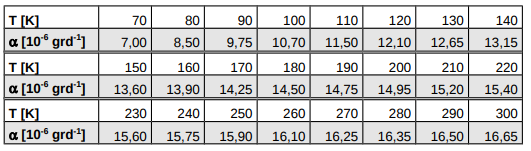
\includegraphics[width=0.8\textwidth]{build/alpha.PNG}
    \caption{$\alpha$ in Abhängigkeit von $T$} %Quelle einfügen
    \label{fig:alpha}
\end{figure}

Dies ergab folgende Werte für die Parameter

\begin{align*}
    a &= (-8, \! 2 \pm 0, \! 7) \cdot 10^{-9} \, \mathrm{K}^{-5} \\
    b &= (7, \! 4 \pm 0, \! 5) \cdot 10^{-6} \, \mathrm{K}^{-4} \\
    c &= (2, \! 5 \pm 0, \! 1) \cdot 10^{-3} \, \mathrm{K}^{-3} \\
    d &= (0, \! 41 \pm 0, \! 02) \, \mathrm{K}^{-2} \\
    e &= (11, \! 3 \pm 0, \! 6) \, \mathrm{K}^{-1}
\end{align*}

und folgenden Plot:

\begin{figure}[H]
    \centering
    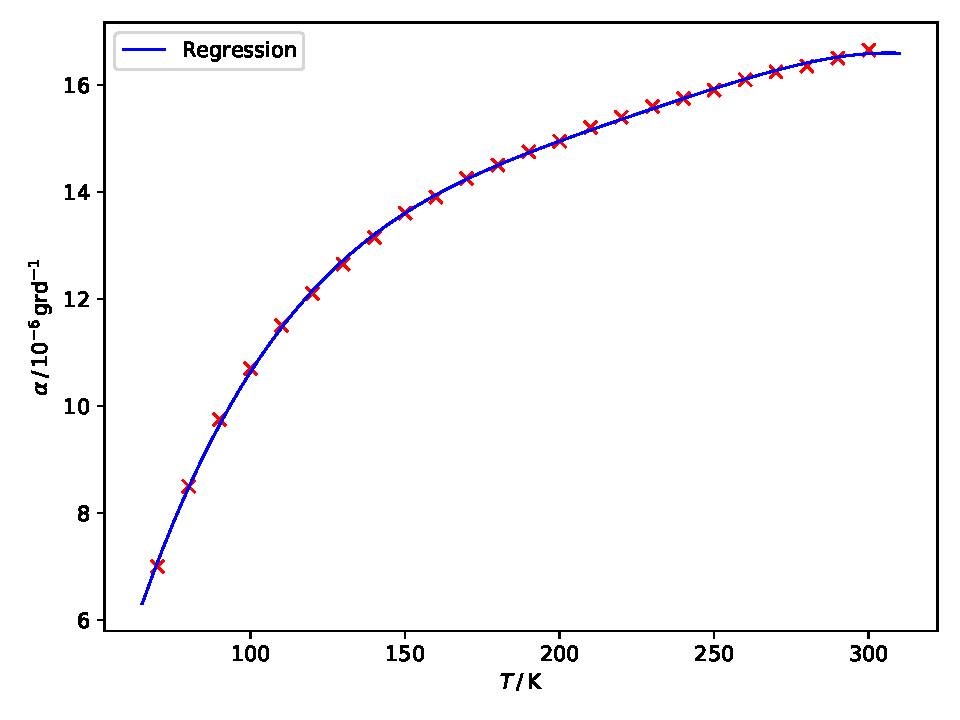
\includegraphics[width=0.8\textwidth]{build/alpha.pdf}
    \caption{$\alpha$ in Abhängigkeit von $T$ mit Ausgleichsrechnung}
    \label{fig:alpha_plot}
\end{figure}

\subsection{Bestimmung der Debye-Temperatur}     %$\theta_D$ noch einfügen :D
\label{sec:debye_temp}

\subsection{Theoretische Bestimmung der Debye-Temperatur}     %$\theta_D$ noch einfügen :D
\label{sec:theo_debye_temp}